\chapter{Diseño y desarrollo\label{sec:disenhoYDesarrollo}}

%\textbf{Rápida intro.}

%TODO: Demostrar todo el dominio que pueda sobre cuestiones de la carrera.

\section{Análisis de requisitos}

\subsection{Análisis funcional}

\begin{rf0}
	\item Creación y gestión de cuestionarios.
	\begin{rf0*}
		\item Creación de preguntas.
		\begin{rf0*}
			\item El profesor debe ser capaz de introducir preguntas al sistema.
		\end{rf0*}
	\end{rf0*}
\end{rf0}

\subsection{Análisis no funcional}


%\textbf{¿Detallar un análisis funcional? Sí}

\section{Diseño}

Los sistemas adaptativos pueden abstrarse como una serie de módulos como los descritos en la figura \ref{fig:diagrama_disenno}. 

\begin{figure}[htp!]
	\centering
	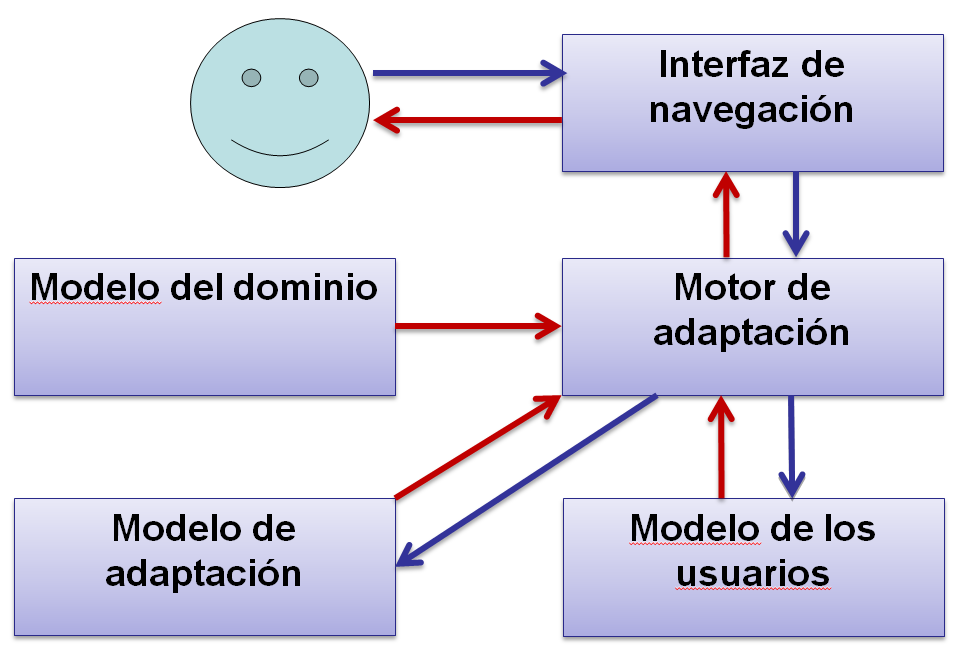
\includegraphics[width=0.75\textwidth,clip=true]{diagrama_disenno}
	\caption{División en módulos de un sistema adaptativo}
	\label{fig:diagrama_disenno}
\end{figure}

El usuario (representado arriba a la izquierda) interacciona con el sistema a través de una interfaz de navegación que representa el estado del motor de adaptación, componente que articula al resto de módulos. El modelo del dominio, de adaptación y el modelo de los usuarios son las herramientas de las que el motor de adaptación obtiene la información que le permite dar una respuesta adecuada a cada situación. Mientras que el modelo del dominio es fijo, en el sentido de que solo ha de definirse durante la creación del sistema y permanece estable durante la vida del mismo, el modelo de adaptación y el modelo de los usuarios van sufriendo variaciones, en función de la entrada que produzcan los usuarios.

Durante las siguientes secciones se dará una descripción más detallada de los módulos.

\subsection{Interfaz de navegación}

La interfaz de navegación es la parte del sistema encargada de permitir la interacción entre el sistema y el usuario. Debe representar ante el usuario la información del sistema que este deba conocer, además de recibir la entrada que el usuario genere para que el motor de adaptación pueda incorporarla.

En el diseño seguido para este trabajo se decidió utilizar las tecnologías web como base sobre la que construir, por lo que las funciones de la interfaz de navegación recaen principalmente en el navegador web del usuario. Aún así, el sistema debe crear y, sobre todo, adaptar los ficheros html que envía al navegador del cliente. Para ello se han utilizado también tecnologías web estándar: HTML, Javascript, CSS y PHP. Más información sobre las tecnologías utilizadas en \ref{sec:tecnologias}.

\subsection{Modelo de los usuarios}

%\textbf{Profesor y estudiante}

El sistema tiene dos roles de usuarios claramente diferenciados: rol docente y rol estudiante. Las necesidades que tienen ambos roles respecto de la aplicación, son radicalmente distintas. Mientras que a los docentes se les debe mostrar herramientas para la creación y gestión de cuestionarios, motorización de resultados y recuperación de exámenes, los estudiantes deben acceder a la ejecución de los cuestionarios, a cierta retroalimentación y a sus resultados.

En ninguno de los dos roles podemos presuponer conocimientos informáticos avanzados, como se recoje en \textbf{Influir cita a RNF}. Además, desde las fases iniciales del proyecto se planteó que el sistema debería ser fácil de usar para docentes y estudiantes de todas las etapas educativas, desde la primera infancia hasta la edad adulta. Al ser una aplicación potencialmente disponible a niños y niñas muy jóvenes, tampoco podemos presuponer que el estudiante sepa leer, debiendo dotar en consecuencia al rol del docente la habilidad de incluir ficheros multimedia con los que suplir dicha carencia.

\subsection{Modelo del dominio}

La aplicación pretende ser una ayuda al aprendizaje y por lo tanto, su dominio es la actividad educativa. Más concretamente, aquellas actividades relacionadas con comprobar, por parte del propio estudiante o de un docente, si el estudiante ha adquirido correctamente ciertos conocimientos. Para ello, a grandes rasgos, el equipo docente de una asignatura creará una serie de preguntas y respuestas, agrupadas por contenidos en materias, que utilizará para crear cuestionarios a los que los estudiantes tendrán acceso. Del resultado de dichos cuestionarios, tanto el estudiante como los docentes podrán conocer cómo están realizando su actividad y realizar los cambios que fueran necesarios.

La asignatura es la primera división que se utiliza normalmente en los entornos educativos. Un docente se encarga de unas asignaturas en concreto y los estudiantes van explorando por asignaturas. Así, cada asignatura tiene asociados un listado de usuarios, algunos comos docentes y otros como estudiantes. Es importante notar que un usuario podría ser docente en una asignatura pero estudiante en otra, por lo que el rol es un atributo de la unión usuario y asignatura, y no solo del usuario.

Dentro de cada asignatura, existen una serie de materias, que son las entidades que clasifican los conocimientos por similitud dentro de una asignatura. El concepto de materia en este modelo se utiliza para representar los conceptos del lenguaje común de \emph{temas} o \emph{partes} en los que se divide una asignatura. Dentro de cada materia existe un cojunto de preguntas, ordenadas por un nivel de relevancia.

La división de las preguntas en niveles de relevancia es una de las características novedosas del modelo propuesto. Con ello se busca facilitar que el estudiante adquiera los conocimientos en el orden más adecuado, asegurando que no se enfrenta a conceptos que dependen de otros hasta que domina los conceptos base. Esta divisón también ayuda a evitar que un estudiante obtenga una buena calificación en un examen porque haya aprendido a realizar los ejercicios, pero aún así carezca de entendimiento sobre los conceptos básicos. Una discusión más detallada sobre el sistema de clasificación de las preguntas en niveles puede encontrarse en el apéndice \ref{apend:preguntas en niveles}.

Cada pregunta lleva asociada una serie de respuestas y solo una es la válida. Tanto las preguntas como las respuestas llevan asociadas mucha información, como el enunciado, imágenes opcionales\ldots En la figura \ref{fig:modelo del dominio} se encuentran detallada toda la información asociada a cada entidad que compone el modelo.

\begin{figure}[htp!]
	\centering
	\includegraphics[width=0.75\textwidth,clip=true]{modelo_dominio}
	\caption{Modelo del dominio}
	\label{fig:modelo del dominio}
\end{figure}

Una vez escrito un número suficiente de preguntas, el equipo docente puede crear cuestionarios. Las cuestionarios pueden ser de autoevaluación para los alumnos o de evaluación clásica, aunque para el sistema son casos idénticos.

%\textbf{Estructura de la BD}

\subsection{Modelo de adaptación}

El sistema contempla dos tipos de adaptación. Primero, tenemos la adaptación de navegación, que es aquella que busca guiar al usuario por el sistema, facilitando su uso. En nuestro caso, la navegación del estudiante es sencilla, por lo que no aplica. Donde sí que es necesario este tipo de adaptación es en el área del docente. A la hora de crear las materias, las preguntas y los cuestionarios existe un orden de trabajo más sencillo que otros y el sistema deberá guiar al usuario por ese recorrido utilizando elementos variables de la interfaz.

El otro tipo de adaptación, la adaptación del contenido, es la más relevante para el sistema. Al igual que la de navegación afecta principalmente al docente, la de contenido afecta sobre todo al estudiante. Las preguntas a las que un estudiante se enfrenta en un cuestionario depende de las respuestas que haya dado a las anteriores.

En concreto, cuando un docente crea un cuestionario establece dos parámetros, $N_l$, que es el número de niveles en los que una pregunta se puede clasificar y $N_v$, que es el número de preguntas que debe responder cada alumno en cada intento del cuestionario. Todos los estudiantes empiezan respondiendo a preguntas del primer nivel y solo se enfrentarán a preguntas de niveles más avanzados cuando hayan respondido correctamente a suficientes preguntas. En concreto, a $\frac{N_v}{N_l}$ preguntas.

\begin{figure}[htp!]
	\centering
	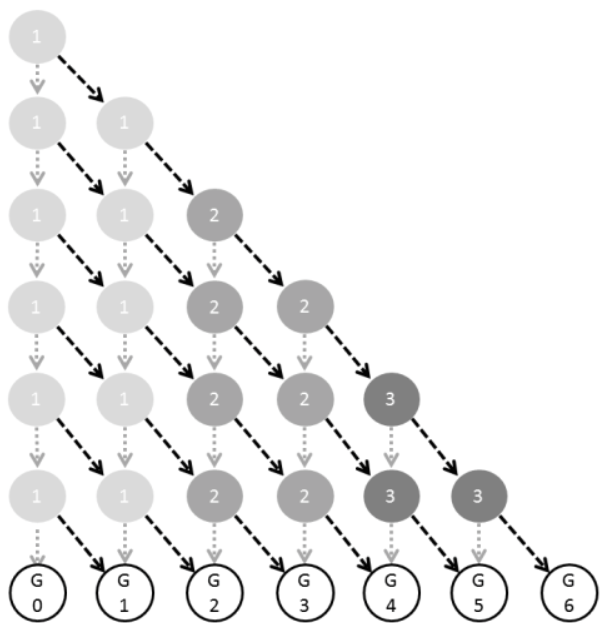
\includegraphics[width=0.75\textwidth,clip=true]{modelo_adaptacion}
	\caption[Modelo de adpatación]{Diagrama que representa todos los posibles recorridos para un cuestionario con $N_l = 3$ y $N_v = 6$. Todos los alumnos entran por la pregunta de la esquina superior izquierda. El número dentro de las circunferencias representa la dificultad de la pregunta. Cuando un alumno responde, toma el camindo de la flecha oscura cuando acierta y de la flecha clara cuando falla. La última fila del diagrama representa las posibles notas que un estudiante puede sacar, ordenadas de menor a mayor de izquieda a derecha.}
	\label{fig:modelo de adaptacion}
\end{figure}

La elección de la siguiente pregunta dentro de un mismo nivel se hace de forma aleatoria, asegurando en todo momento que no haya preguntas repetidas dentro del mismo cuestionario. Cuando el alumno sube de nivel, ya solo responde a preguntas de ese nuevo nivel. Como el número de preguntas está limitado, es posible que un estudiante no llegue a responder preguntas de todos los niveles o incluso puede que solo responda preguntas del primer nivel. Una vez que se ha subido de nivel, no se puede bajar, aunque cada vez que se repita el cuestionario se volverá al primer nivel.

Que la respuesta de una pregunta condicione la siguiente pregunta obliga a que el estudiante responda a cada pregunta, a diferencia de los cuestionarios clásicos, donde una pregunta puede dejarse sin respuesta y continuar con la siguiente. Para solucionar esta diferencia el equipo docente puede establecer que exista una opción adicional de respuesta que indique que el alumno no conoce la respuesta que el sistema tratará como respuesta incorrecta a la hora de seleccionar la siguiente pregunta. Así mismo, la aplicación da al docente la opción de mostrar una casilla que especifique que el alumno ha respondido sin estar seguro de que sea la respuesta correcta. Más información sobre el modelo del examen, en concreto sobre el sistema de calificación, puede encontrarse en el apéndice \ref{apen:como se ponen las notas}

Por último, el docente puede decidir que los estudiantes reciban feedback al responder una pregunta o no. Si lo hacen, cuando el alumno responda se indicará si la respuesta es correcta o no, además de un mensajes de feedback escrito por el profesor para cada pregunta.


%\textbf{Exámenes con distintos niveles y cómo se pasa de uno a otro. Hablar también del feedback o del no lo sé}



% Susection a ignorara
%\subsection{Motor de adaptación}

%\textbf{Rápidas notas sobre la aplicación en sí. O no.}





\section{Desarrollo: e-valUAM\label{sec:desarrollo}}

En esta sección se detalla cómo se ha implementado el proyecto, tomando como referencia lo expuesto en las secciones anteriores.

\subsection{Visión general}

\subsection{Tecnologías y lenguajes empleados\ref{sec:tecnologias}}

\subsection{Módulos asociados al docente}

\subsection{Módulos asociados al estudiante}

%\textbf{En la introducción dejar muy claro qué se ha desarrollado y qué no se ha desarrollado.}
